\section{Introduzione}
Il presente elaborato è stato scritto per il superamento dell'esame Ingegneria Del Software del corso di laurea triennale in Ingegneria Informatica dell'Università degli Studi di Firenze.\newline
Si descrive il design e l'implementazione in \textit{Java} di un sistema gestionale per biblioteche. \newline

Il progetto è stato versionato usando Git e l'intero codice sorgente è disponibile all'url \url{https://github.com/salvatore-greco/SWE}. Sono state usate due GitHub Action per gestire il deploy su GitHub Pages dei risultati di coverage e per la compilazione della presente relazione.


\subsection{Statement}
Il progetto modella un sistema di gestione per biblioteche comunali, prendendo d'ispirazione le biblioteche del comune di Firenze.
Il sistema permette la gestione da parte del personale della biblioteca del proprio catalogo di libri permettendone l'aggiunta, la modifica e la cancellazione. Semplifica le operazioni di prestito permettendo agli utenti di prenotare una copia da prendere successivamente in biblioteca; essa deve essere approvata dal bibliotecario per registrarne l'effettivo prestito; inoltre può essere effettuato anche senza prenotazione, recandosi in biblioteca e registrandone il prestito dal bibliotecario. Permette inoltre di gestire eventi, come mostre di libri, incontri con gli autori, mostrando dettagli sulla data, luogo e durata dell'evento e permettendo agli utenti di riservare un posto nell'aula. 
I servizi offerti sono disponibili attraverso la richiesta della tessera della biblioteca. L'utente sprovvisto di tessera, ma provvisto di credenziali può farne richiesta, presentandosi poi in biblioteca per il suo rilascio fisico tramite il bibliotecario.
L'amministratore della biblioteca può gestirne il budget e il catalogo attraverso le operazioni CRUD sui libri descritte precedentemente.
Se provviste di aule studio, ne permette la gestione: consultare i posti disponibili  e prenotarne uno; essi vengono rilasciati in modo automatico giornalmente e possono essere rilasciati manualmente da parte degli utenti.    

\subsection{Architettura e tecnologie utilizzate}\label{subsec:architettura}
Per lo sviluppo è stato utilizzato \textit{Java}, utilizzando come IDE \textit{IntelliJ} data la sua grande integrazione con l'ecosistema e col database.
Come database è stato scelto \textit{PostgreSQL}, utilizzando le API \textit{JDBC} e il suo relativo driver. Use Case Diagram e Class Diagram seguono lo standard UML e sono stati realizzati col software \textit{StarUML}.\newline
Sono state usate le seguenti dipendenze esterne, gestite attraverso il build system \textit{Maven}:
\begin{itemize}
    \item \textbf{PostgreSQL JDBC driver}
    \item \href{https://github.com/cdimascio/dotenv-java}{\textbf{dotenv-java}}: per la gestione delle variabili d'ambiente in file \textit{.env} per il collegamento al database
    \item \textbf{spring-security-crypto}: per l'hashing delle password attraverso l'algoritmo \textit{Bcrypt}
    \item \textbf{JUnit}
    \item \textbf{spring-jdbc}: per l'esecuzione di script da file \textit{.sql}. Usato per l'inizializzazione e la pulizia del database nello schema test.
    \item \textbf{Mockito}: per la creazione di mock e stub per Unit Testing.
    \item \textbf{JaCoCo}: per statistiche di copertura dei test.
\end{itemize}
Il progetto è stato diviso in quattro package: DomainModel, BusinessLogic, ORM, Exception.\newline
Per la business logic è stato scelto di creare un controller per attore data l'assenza di una GUI. Data questa circostanza è stato scritto un ampio numero di test case, fra Unit Test e Integration Test.
\begin{figure}[H]
    \centering
    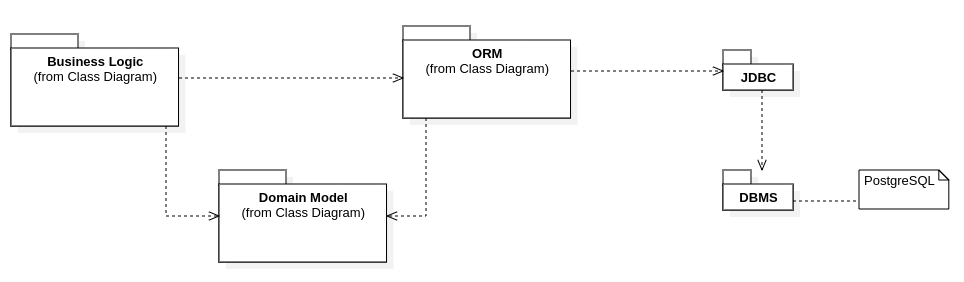
\includegraphics[width=1\linewidth]{images/package_diagram.png}
    \caption{Package diagram del progetto}
    \label{fig:placeholder}
\end{figure}